\graphicspath{{images/}}

\section{Results}

\subsection{Overall Summary}

The overall results from testing the custom and blackbox models for the three classifiers are summarized in ~\autoref{tab:model_winners}:

\begin{table}[H]
  \centering
  \caption{Overall Testing Results}
  \label{tab:model_winners}
  \begin{tabularx}{0.85\textwidth}{X|X}
    \toprule
    \textbf{Model}               & \textbf{Winner}       \\
    \midrule
    Decision Tree Classifier     & Custom Implementation \\
    Random Forest Classifier     & Scikit-Learn Blackbox \\
    Gradient Boosting Classifier & Scikit-Learn Blackbox \\
    \bottomrule
  \end{tabularx}
\end{table}
\FloatBarrier

\textbf{The code for the tests conducted below are found in the \textit{scratch.ipynb} file attached along with this submission.}

\textbf{Overall, the tests of the custom classifiers seem to echo the theoretical understanding that the Gradient Boosting method performs the best, followed by Random Forest Models and simple Decision Trees}. The specifics of the testing process as well as the performance of each classifier are discussed in the subsequent subsections:

\subsection{Testing Approach}

The custom implementations of the decision tree, random forest and gradient boosting classifiers were trained and tested on a dataset generated using the \texttt{scikit-learn} package's \texttt{make\_classification} dataset. The specifics of the generated dataset are summarized in ~\autoref{tab:dataset_params}:

\begin{table}[H]
  \centering
  \begin{tabularx}{0.65\textwidth}{X|X}
    \toprule
    \textbf{Parameter}           & \textbf{Value} \\
    \midrule
    Number of Samples            & 1000           \\
    Number of Features           & 30             \\
    Number of Classes            & 2              \\
    Number of Clusters per Class & 1              \\
    \texttt{n\_informative}      & 15             \\
    \bottomrule
  \end{tabularx}
  \caption{Dataset Parameters}
  \label{tab:dataset_params}
\end{table}
\FloatBarrier

The dataset was split into testing and training datasets in an 80-20 split, leading to 800 training samples and 200 testing samples.

\subsubsection{Decision Tree Classifier}

The custom model and the scikit-learn model were both initialized with the same hyperparameters described below:

\begin{table}[h!]
  \centering
  \begin{tabularx}{0.65\textwidth}{X|X}
    \toprule
    \textbf{Parameter}        & \textbf{Value} \\
    \midrule
    Maximum Depth             & 5              \\
    Maximum Features          & 7              \\
    Minimum Samples to Split  & 15             \\
    Minimum Impurity Decrease & 0.001          \\
    \bottomrule
  \end{tabularx}
  \caption{Decision Tree Model Parameters}
  \label{tab:dt_modelparams}
\end{table}

The results from training both of the models on the dataset are summarized in ~\autoref{tab:dt_model_performance}:

\begin{table}[h!]
  \centering
  \begin{tabular}{lcc}
    \toprule
              & \textbf{Custom Implementation} & \textbf{Scikit-Learn Blackbox Implementation} \\
    \midrule
    Accuracy  & 0.86                           & 0.85                                          \\
    Precision & 0.86                           & 0.85                                          \\
    Recall    & 0.86                           & 0.85                                          \\
    F1 Score  & 0.86                           & 0.85                                          \\
    \bottomrule
  \end{tabular}
  \caption{DT Models - Performance}
  \label{tab:dt_model_performance}
\end{table}

From the above summary, it can be seen that the \textbf{custom model} performed slightly better than the \textbf{scikit-learn blackbox} implementation.

The custom implementation of the decision tree can be seen in ~\autoref{fig:dt_custom_tree}.

\begin{figure}[H]
  \centering
  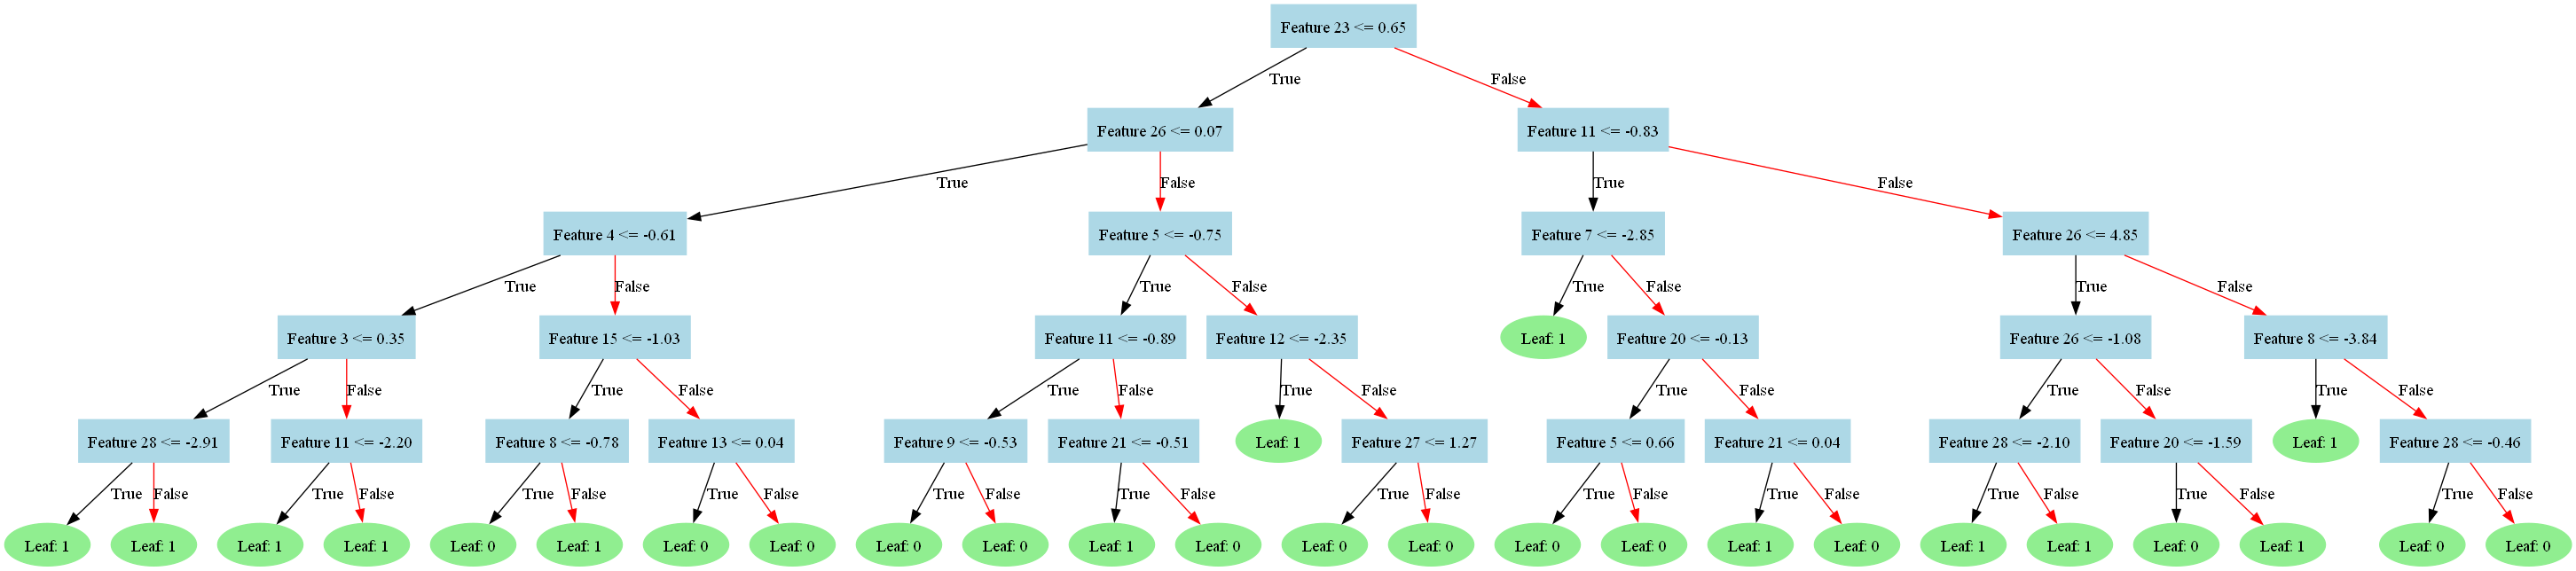
\includegraphics[width=0.9\textwidth]{tree_visualization.png}
  \caption{Custom Decision Tree}
  \label{fig:dt_custom_tree}
\end{figure}
\FloatBarrier

\subsubsection{Random Forest Classifier}

The custom model and the scikit-learn model were both initialized with the same hyperparameters described below:

\begin{table}[H]
  \centering
  \begin{tabular}{lc}
    \toprule
    \textbf{Parameter}        & \textbf{Value} \\
    \midrule
    Number of Estimators      & 100            \\
    Maximum Depth             & 5              \\
    Maximum Features          & 7              \\
    Minimum Samples to Split  & 15             \\
    Minimum Impurity Decrease & 0.001          \\
    \bottomrule
  \end{tabular}
  \caption{RF Model Parameters}
  \label{tab:rf_modelparams}
\end{table}

The results from training both of the models on the dataset are summarized in ~\autoref{tab:rf_model_performance}:

\begin{table}[H]
  \centering
  \begin{tabular}{lcc}
    \toprule
              & \textbf{Custom Implementation} & \textbf{Scikit-Learn Blackbox Implementation} \\
    \midrule
    Accuracy  & {0.92}                         & 0.95                                          \\
    Precision & {0.92}                         & 0.95                                          \\
    Recall    & 0.92                           & {0.94}                                        \\
    F1 Score  & 0.91                           & {0.95}                                        \\
    OOB Score & 0.93                           & {0.95}                                        \\
    \bottomrule
  \end{tabular}
  \caption{RF Models - Performance}
  \label{tab:rf_model_performance}
\end{table}

As mentioned before, around one-third of the observations are left out when fitting a bagged tree. These observations are called \textbf{Out-Of-Bag} observations (\textbf{OOB} for short). The \textbf{OOB Score} in the above table refers to the percentage of correct predictions made on OOB samples taken for validation.

Both the custom implementation as well as the blackbox implementation have high OOB scores, meaning both of the models performed well on predicting the class associated with out-of-bag samples. However, the \textbf{scikit-learn blackbox} model came on top with an OOB Score of 95\% compared to the 93\% of the custom implementation.

A similar trend is seen across the other metrics as well, with the \textbf{scikit-learn blackbox} model having a slight edge over the \textbf{custom model}. However, it should be noted that the custom model has performed extremely well.

\subsubsection{Gradient Boosting Classifier}

\begin{table}[H]
  \centering
  \begin{tabular}{lc}
    \toprule
    \textbf{Parameter}        & \textbf{Value} \\
    \midrule
    Number of Estimators      & 100            \\
    Learning Rate             & 0.3            \\
    Maximum Depth             & 5              \\
    Maximum Features          & 7              \\
    Minimum Samples to Split  & 15             \\
    Minimum Impurity Decrease & 0.001          \\
    \bottomrule
  \end{tabular}
  \caption{GB Model Parameters}
  \label{tab:gb_modelparams}
\end{table}

The results from training both of the models on the dataset are summarized in ~\autoref{tab:gb_model_performance}:

\begin{table}[H]
  \centering
  \begin{tabular}{lcc}
    \toprule
              & \textbf{Custom Implementation} & \textbf{Scikit-Learn Blackbox Implementation} \\
    \midrule
    Accuracy  & 0.92                           & 0.96                                          \\
    Precision & 0.92                           & 0.96                                          \\
    Recall    & 0.92                           & 0.96                                          \\
    F1 Score  & 0.92                           & 0.96                                          \\
    \bottomrule
  \end{tabular}
  \caption{GB Models - Performance}
  \label{tab:gb_model_performance}
\end{table}

The scikit-learn blackbox implementation of the Gradient Boosting Classifier consistently outperformed the custom model across multiple evaluation criteria, including accuracy, precision, recall, and F1 score. These findings underscore the effectiveness and robustness of the scikit-learn Gradient Boosting model in capturing complex relationships within the dataset.